\documentclass{article}
\usepackage[utf8]{inputenc}
\usepackage{natbib}
\usepackage{url}
\usepackage{graphicx}
\usepackage{caption}
\usepackage[a4paper, margin=1.0cm]{geometry}

\title{
    iHP-Emulator Module
\\
\begin{small}
    Joint Honours Project Plan
\end{small} 
}

\author{Sonke Wohler \\
\begin{small}
    s.wohler.15@aberdeen.ac.uk
\end{small}
}
\date{\begin{small}
    Department of Computing Science/ Department of Physics
    \\
    University of Aberdeen
\end{small}}

\pagestyle{empty}

%\bibliographystyle{unsrt}
%\bibliographystyle{abbrv}
\bibliographystyle{plain}
%\bibliographystyle{apalike}

%********************************************************************************

\begin{document}

\maketitle
\thispagestyle{empty}

\section{Context of the Project}
Automation and the innovative use of Computer Technology has become an indispensable tool in keeping up with competition in many industries today. However, Safety Critical Industries at times remain rather conservative in adapting new technologies and as a result are unable to take advantage of numerous opportunities. Chief among these may be the Oil and Gas Industry, with Billions of Dollars worth of equipment and material at risk, as well as human lives, innovation comes second to robust and proven technologies. \cite{chickenEgg,cloudOil}

\subsection{The iHP}
One of the many processes that could be further automated in the Industry is the Injection of mono-ethylene-glycol (MEG) or other anti-freezing agents in sub-sea Gas Production Fields. Here the significant water-content in the extracted gas, at the low sea-bed temperatures, frequently causes issues when freezing and capturing Gas Molecules in the process. Hydrate Formation, as it is called, can pose a serious danger to production and even safety.\cite{dataBook,gasBook,hydrateFormation}
\\\\The Intelligent Hydrate Project (iHP) aims to provide an Automated Solution to the Problem of Hydrates, making use of state of the art Machine Learning Technology. As part of this Project it has become increasingly evident that some form of Emulation of the real world situation is required both for in depth System testing and to provide essential Data for the Machine Learning aspects of the System. For this purpose a minimalist Emulator Module has been designed over the past summer, but as the System progresses and the Project grows the Emulator also has to progress to remain relevant to the current state of the System.

\section{The Project}
This Undergraduate Project aims to produce a meaningful improvement on the existing Emulator Module currently used in the iHP. It is an attempt to make use of the Physical Expertise of the student in the Software Development Environment.
\\\\For this purpose sub-sea Processes should be emulated as possible, based on a qualitative Physical Model of the Gas Production. This Model should represent a meaningful approximation of the Thermodynamics and Fluid Mechanics that define the sub-sea processes and should produce a significant improvement over the existing Emulator Module.
\\\\ This Physical Model is then to be integrated as a real time Emulator Module into the iHP. As such it must be engineered in line with the Architectural Patterns of the larger Industrial Project and provide a real time representation for the User to interact with. At the completion of this Honours Project the Module must be shown to fulfil set out requirements through strategic testing.

\subsection{Requirement Specifications}
The Student is aiming to fulfil the following goals:

\begin{enumerate}
    \item (Must Have) A Qualitative Physical Model to represent sub-sea production processes.
    \item (Must Have) A Knowledge Representation to be used in the iHP. (note: This will heavily affect other aspects of the iHP.)
    \item (Must Have) A Software Module Incorporating the above.
    \item (Must Have) Compliance with Software Development Practice for Quality Assurance, as laid out in the iHP, and compliance with its requirements and Specifications were possible.
    \item (Should Have) Integration of this Module with the iHP, including real time emulation for Usability testing.
    \item (Could Have) As required and possible: Adaptations to the iHP to facilitate integration and reflect Knowledge Representation, in particular in inter-operational aspects but also graphical-interface and other aspects.
\end{enumerate}


\subsection{Proposed Project Time-line}

\begin{figure}[h]
    \centering
    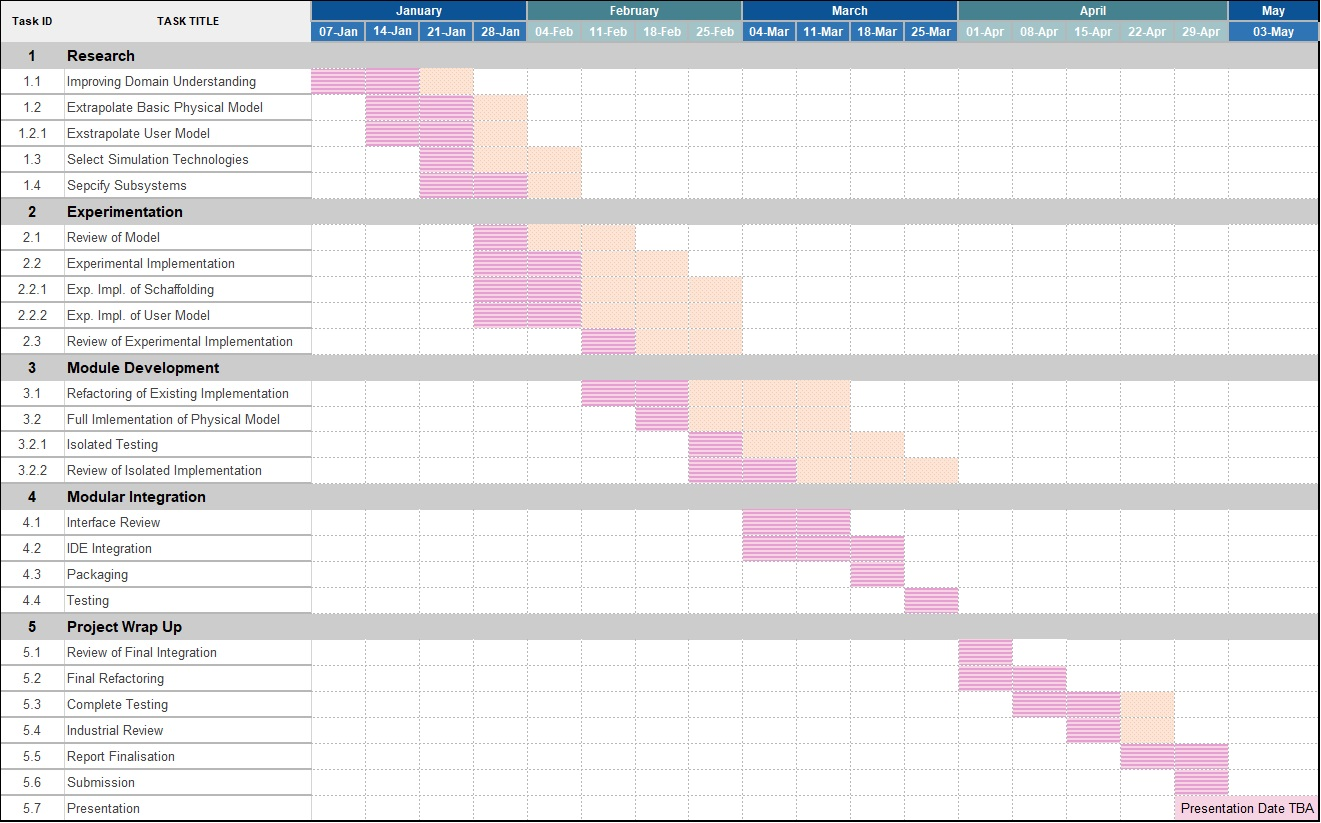
\includegraphics[width=\linewidth]{ProjectPlan.jpg}
    \caption{Gantt Chart of a time-line that aims to deliver on the above specified goals, with best case time-line in pink and worst case time-line in orange.
    Note that Phase 4 (Integration) may have to be left out in the worst case.
    }
    \label{fig:gantt}
\end{figure}

\subsection{Risk Factors and Other Considerations}
Part of the motivation for this Honours Project is to produce Data that is otherwise inaccessible to the industrial team. Earlier attempts to acquire real Data or Domain Knowledge have proven difficult with very limited success. An Emulator Module set out to tackle this issue would also be impacted by the same which could could limit the possible success of the Project.
\\\\Another possible issue is the requirement for real time interaction. Most meaningful simulations are computed over a longer time-span as only the Data produced is required, but for the iHP User Interaction will become an important aspect for Usability testing, presentation and for basic security demonstrations. This places constraints on the Physical Model as much as it requires efficient design to achieve this requirement.
\\\\As such the Core of the Project is a meaningful and well developed Emulation while integration goals can be met outside of the Honours Project should development be stalled.
\\\\As a semi-industrial Project the Hardware and Software required by the student is already sufficiently supplemented by the iHP Project.








\clearpage
\nocite{gasBook,dataBook,cloudOil,chickenEgg,hydrateFormation}
\bibliography{refs}

\end{document}
